Nel contesto dei casi d'uso, un attore è colui che interagisce con il sistema per ottenere un obiettivo specifico.\\
La {\hyperref[fig:attori-casi-duso]{Figura 3.2}} mostra uno schema contenente tutti gli attori del sistema, i dettagli di ciascun attore sono descritti di seguito:

\subsection*{Utente non autenticato:}

\begin{itemize}
    \item \textbf{Descrizione:}  L'utente non autenticato è una persona che sta cercando di accedere al sistema, ma non ha effettuato il \textit{login}.\\
    Non ha accesso ai dati sensibili o alle funzionalità avanzate riservate agli utenti autenticati;
    \item \textbf{Ruolo:} Questo attore ha il compito di interagire con il sistema senza diritti di accesso completi.\\
    Il suo obiettivo principale è autenticarsi per diventare un utente con pieno accesso al sistema;
    \item \textbf{Attività principali:}
        \begin{itemize}
            \item Effettuare il \textit{login} con le proprie credenziali;
            \item Visualizzare i messaggi di errore in caso di \textit{login} fallito.
        \end{itemize}
\end{itemize}

\subsection*{Utente autenticato:}

\begin{itemize}
    \item \textbf{Descrizione:}  L'utente autenticato è una persona che ha effettuato il \textit{login} con successo ed ha accesso completo alle funzionalità del sistema.\\
    Può cercare, filtrare, visualizzare, generare e rigenerare i progetti;
    \item \textbf{Ruolo:} Questo attore può eseguire operazioni avanzate, come la generazione di progetti, il salvataggio delle bozze ed il \textit{download} dei progetti in formato PDF;
    \item \textbf{Attività principali:}
        \begin{itemize}
            \item Visualizzare e cercare progetti;
            \item Generare e rigenerare progetti;
            \item Salvare e visualizzare bozze;
            \item Visualizzare e scaricare progetti in formato PDF.
        \end{itemize}
\end{itemize}

\subsection*{\textit{Large language models}:}

\begin{itemize}
    \item \textbf{Descrizione:}  L'attore \gls{llm} è un sistema automatizzato di generazione dei contenuti, che utilizza algoritmi avanzati di \gls{aig} per generare e rigenerare progetti o singoli capitoli di progetti. \\
    Il \gls{llm} è responsabile dell'elaborazione delle richieste degli utenti e della generazione automatica del contenuto tecnico dei progetti;
    \item \textbf{Ruolo:}  Il \gls{llm} è un componente del sistema che esegue la generazione di contenuti complessi in modo autonomo.\\
    La sua funzione principale è rispondere alle richieste dell'utente riguardo la creazione e la rigenerazione di progetti;
    \item \textbf{Attività principali:}
        \begin{itemize}
            \item Ricevere richieste di generazione di progetti da parte degli utenti;
            \item Generare contenuti basati su preset predefiniti;
            \item Rigenerare progetti o singoli capitoli in risposta a richieste di aggiornamento;
            \item Restituire i contenuti generati all'utente.
        \end{itemize}
\end{itemize}

\begin{figure}[H]
    \centering
    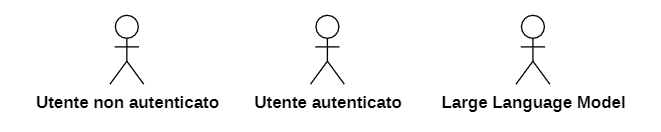
\includegraphics[width=1\textwidth]{usecase/attori.png}
    \caption{Attori dei casi d'uso}
    \label{fig:attori-casi-duso}
\end{figure}


